\documentclass[11pt]{article}
\usepackage[utf8]{inputenc}
\usepackage[T1]{fontenc}
\usepackage{lmodern}
\usepackage{geometry}
\usepackage{tikz}
\usetikzlibrary{arrows.meta,shapes.geometric}

\geometry{paperwidth=16cm,paperheight=5.0cm,margin=0cm}
\pagestyle{empty}
\setlength{\parindent}{0pt}

\definecolor{ctxFill}{RGB}{238,242,245}
\definecolor{ctxLine}{RGB}{155,168,179}
\definecolor{ctxText}{RGB}{38,52,67}
\definecolor{exFill}{RGB}{220,233,247}
\definecolor{exLine}{RGB}{23,54,93}
\definecolor{prFill}{RGB}{200,240,236}
\definecolor{prLine}{RGB}{8,127,140}
\definecolor{prText}{RGB}{6,79,87}

\begin{document}
\noindent
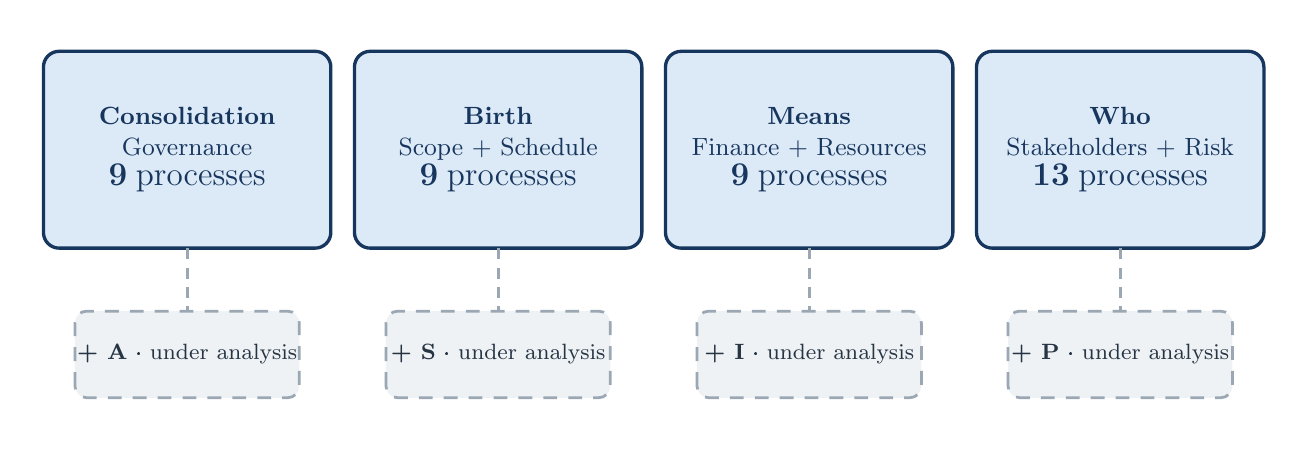
\begin{tikzpicture}[x=1cm,y=1cm,font=\small]
  \path[use as bounding box] (0,0) rectangle (16,5.0);
  \draw[fill=exFill,draw=exLine,line width=1.2pt,rounded corners=0.2cm] (0.2,2.2) rectangle (3.85,4.7);
  \node[align=center,text width=3.4cm,text=exLine] at (2.025,3.45) {\textbf{Consolidation}\\ Governance\\ \large\textbf{9} processes};
  \draw[fill=ctxFill,draw=ctxLine,line width=1pt,dash pattern=on 5pt off 4pt,rounded corners=0.15cm] (0.6000000000000001,0.3) rectangle (3.45,1.4);
  \node[align=center,text=ctxText] at (2.025,0.85) {\footnotesize\textbf{+ A} · under analysis};
  \draw[draw=ctxLine,line width=1pt,dash pattern=on 4pt off 3pt] (2.025,2.2) -- (2.025,1.4);
  \draw[fill=exFill,draw=exLine,line width=1.2pt,rounded corners=0.2cm] (4.15,2.2) rectangle (7.800000000000001,4.7);
  \node[align=center,text width=3.4cm,text=exLine] at (5.9750000000000005,3.45) {\textbf{Birth}\\ Scope + Schedule\\ \large\textbf{9} processes};
  \draw[fill=ctxFill,draw=ctxLine,line width=1pt,dash pattern=on 5pt off 4pt,rounded corners=0.15cm] (4.550000000000001,0.3) rectangle (7.4,1.4);
  \node[align=center,text=ctxText] at (5.9750000000000005,0.85) {\footnotesize\textbf{+ S} · under analysis};
  \draw[draw=ctxLine,line width=1pt,dash pattern=on 4pt off 3pt] (5.9750000000000005,2.2) -- (5.9750000000000005,1.4);
  \draw[fill=exFill,draw=exLine,line width=1.2pt,rounded corners=0.2cm] (8.1,2.2) rectangle (11.75,4.7);
  \node[align=center,text width=3.4cm,text=exLine] at (9.924999999999999,3.45) {\textbf{Means}\\ Finance + Resources\\ \large\textbf{9} processes};
  \draw[fill=ctxFill,draw=ctxLine,line width=1pt,dash pattern=on 5pt off 4pt,rounded corners=0.15cm] (8.5,0.3) rectangle (11.35,1.4);
  \node[align=center,text=ctxText] at (9.924999999999999,0.85) {\footnotesize\textbf{+ I} · under analysis};
  \draw[draw=ctxLine,line width=1pt,dash pattern=on 4pt off 3pt] (9.924999999999999,2.2) -- (9.924999999999999,1.4);
  \draw[fill=exFill,draw=exLine,line width=1.2pt,rounded corners=0.2cm] (12.05,2.2) rectangle (15.700000000000001,4.7);
  \node[align=center,text width=3.4cm,text=exLine] at (13.875,3.45) {\textbf{Who}\\ Stakeholders + Risk\\ \large\textbf{13} processes};
  \draw[fill=ctxFill,draw=ctxLine,line width=1pt,dash pattern=on 5pt off 4pt,rounded corners=0.15cm] (12.450000000000001,0.3) rectangle (15.3,1.4);
  \node[align=center,text=ctxText] at (13.875,0.85) {\footnotesize\textbf{+ P} · under analysis};
  \draw[draw=ctxLine,line width=1pt,dash pattern=on 4pt off 3pt] (13.875,2.2) -- (13.875,1.4);
\end{tikzpicture}
\end{document}
